\documentclass[conference]{IEEEtran}

\usepackage{cite}
\usepackage[pdftex]{graphicx}
\graphicspath{{figures/}}
\usepackage[cmex10]{amsmath}
\usepackage{algorithmic}
\usepackage{algorithm}
\usepackage{array}
\usepackage{fixltx2e}
\usepackage{stfloats}
\usepackage{url}
\usepackage{amssymb}
\usepackage{float}
\usepackage{color}

\newcommand{\norm}[1]{\left\lVert #1 \right\rVert}

\begin{document}

\title{Parallel Stochastic Gradient Descent for Stacked Autoencoders}

\author{\IEEEauthorblockN{Jason Liang}
\IEEEauthorblockA{jasonzliang@utexas.edu}
\and
\IEEEauthorblockN{Keith Kelly}
\IEEEauthorblockA{keith@ices.utexas.edu}}

\maketitle

\begin{abstract}
The abstract goes here.
\end{abstract}

\section{Introduction}
Autoencoders are a method for performing representation learning, a process during which a more useful representation of the
input data is automatically determined. Representation learning is important in machine learning since ``the performance of 
machine learning methods is heavily dependent on the choice of data representation (or features) in which they are applied" 
\cite{bengio2012rep}. An autoencoder is a neural network in which the output layer and the input layer have the same size,
so that the original input can be used to determine how well or how poorly the autoencoder encodes the data. Consider a 
neural network with one hidden layer and one output layer which has the same size as the input layer. Suppose
that the input $x\in\mathbb{R}^m$ (and the output as well) and suppose that the hidden layer has $n$ nodes. Then we
have a weight matrix $W\in\mathbb{R}^{m\times n}$ and bias vectors $b$ and $b^{'}$ in $\mathbb{R}^m$ and $\mathbb{R}^n$, respectively.
Let $s(x) = 1/(1+e^{-x})$ be the sigmoid (logistic) transfer function. Then we have a neural network as shown in \ref{fig:autoencoder}.
We want that $n<m$ so that the learned representation of the input exists in a lower dimensional space than the input. The output
can be considered a prediction of the input given the code in the hidden layer. We can then determine how well the autoencoder
encodes (and then decodes) the data by comparing input to the output. If they are similar, then the code in the hidden layer
represents a good, lower dimensional representation of the input data.


\begin{figure}[h]
\centering
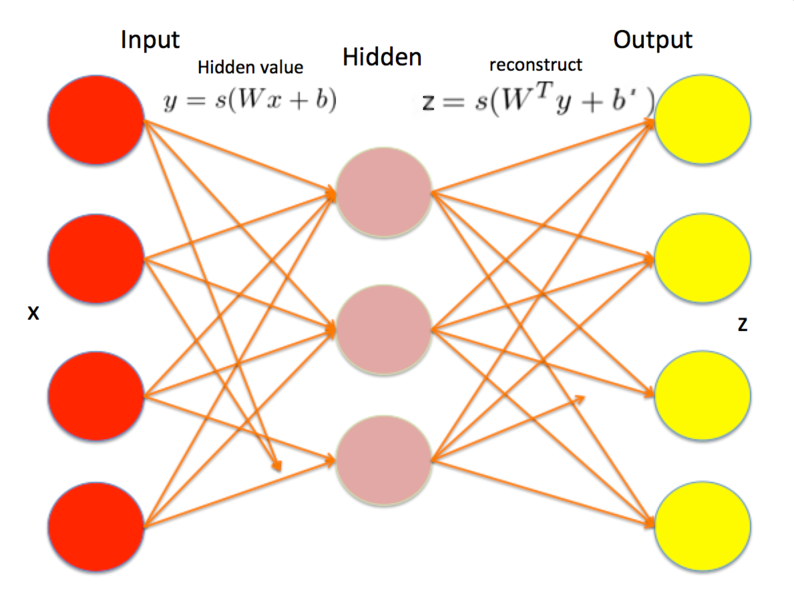
\includegraphics[width=0.9\linewidth]{autoencoder.png}
\caption{autoencoder}
\label{fig:autoencoder}
\end{figure}

\section{Related Work}
related work here, cite like this \cite{vincent2010stacked}

\section{Algorithm Description}
We start with a random weight matrix $W$ and random biases $b$ and $b^{'}$. We take a given input $x$, and feed it forward through the network and 
compute the error between the target output $t$ and the actual output $z$. Often we use the squared loss error $E(t,z) = \frac{1}{2}\norm{t-z}_2^2$ to determine the difference
between the two. In the case of an autoencoder, the target output is the same as the input. If the error is not satisfactory, we can adjust the weight matrix and that biases in order to attempt to learn a better representation
of the data. A common method of updating the weight and biases is via backpropogation. We can use gradient descent to update the weights and biases. We
will first consider the update for the weights and biases from the last hidden layer to the output layer with a squared loss error function and derive the updates. 
We use as an example a simple three layer neural network (one input, one hidden and one output node). Some notation:

\begin{table}[h]
\normalsize
\begin{tabular}{l|l}
Symbol     & Meaning                                                          \\ \hline
$E$          & Error as computed at the output layer                            \\
$x_j$       & Node $j$ in the input layer                                      \\
$y_j$       & Node $j$ in the hidden layer                                     \\
$z_j$       & Node $j$ in the output layer                                     \\
$n_j$       & $\sum_{i=1}^n W_{ij}x_i + b_j$                                   \\
$t_j$       & Target output at node $j$                                   \\
$W_{ij}^H$ & Weight $i,j$ from input to hidden layer \\
$W_{ij}^O$ & Weight $i,j$ from hidden to output layer \\
$s(x_j)$    & $1/(1+e^{-x_j})$                                                 
\end{tabular}
\end{table}

The derivative of the output error $E$ with respect to an output matrix weight $W_{ij}^O$ is as follows.

\begin{equation}
\begin{split}
\frac{\partial E}{\partial W^O_{ij}} &= \frac{\partial E}{\partial z_j}\frac{\partial z_j}{\partial W^O_{ij}} \\
																	 &=(z_j - t_j)\frac{\partial s(n_j)}{\partial x_j}\frac{\partial x_j}{\partial W^O_{ij}} \\
																	 &=(z_j-t_j)s(n_j)(1-s(n_j))x_i \\
																	 &=(z_j-t_j)z_j(1-z_j)x_i \\
\end{split}
\label{}
\end{equation}
Now that we have the gradient for the error associated to a single training example, we can compute the updates.
\begin{equation}
\begin{split}
\delta^O_j &= (z_j-t_j)z_j(1-z_j) \\
W^O_{ij} &\leftarrow W_{ij} - \eta \delta^O_j x_i \\
b_j &\leftarrow b_j - \eta\delta_j
\end{split}
\end{equation}

The computation of the gradient for the weight matrix between hidden layers is simiilarly easy to compute.
\begin{equation}
\begin{split}
\frac{\partial E}{\partial W^H_{ij}} &= \frac{\partial E}{\partial y_j}\frac{\partial y_j}{\partial W^H_{ij}} \\
																	 &=\left(\sum_{k=1}^m \frac{\partial E}{\partial z_k}\frac{\partial z_k}{\partial n_k}\frac{\partial n_k}{\partial y_j} \right)\frac{\partial y_j}{\partial n_j}\frac{\partial n_j}\partial W_{ij}^H\\
																	 &=\left(\sum_{k=1}^m (z_k - t_k)(1-z_k)z_kW_{jk}^O \right)y_j(1-y_j)x_i
\end{split}
\label{}
\end{equation}
And then using the computed gradient we can define the updates to be used for the hidden layers
\begin{equation}
\begin{split}
\delta^H_j &= \left(\sum_{k=1}^m (z_k - t_k)(1-z_k)z_kW_{jk}^O \right)y_j(1-y_j) \\
W^H_{ij} &\leftarrow W^H_{ij} - \eta\delta^H_jx_i \\
b_j &\leftarrow b_j - \eta\delta^H_j
\end{split}
\end{equation}

In general, for a neural network we may have different output error function and these will result in different update rules. We will also give the updates
for the cross-entropy error function with softmax activation in the final layer.
The cross entropy error function is given by $E(x,t) = -\sum_{i=1}^n \left(t_i\ln z_i + (1-t_i)\ln(1-z_i)\right)$
and the softmax function is given by $\sigma(x_j) = e^{x_j} /(\sum_k e^{x_k})$. Following the same procedure as above
for computing the gradient and the updates, we find that for hidden/output layer

\begin{equation}
\begin{split}
\frac{\partial E}{\partial W^O_{ij}} &= (z_j - t_j)y_i \\
\delta^O_j &= (z_j-t_j) \\
W^O_{ij} &\leftarrow W_{ij} - \eta \delta^O_j x_i \\
b_j &\leftarrow b_j - \eta\delta_j.
\end{split}
\end{equation}

Note also that we find that the updates for the input/hidden layer is the same as in the squared error loss function with sigmoid activation.

The algorithm and derivations for the autoencoder (a special type of neural network) are a slight variation on the above derivations
for a more general neural network.

We give the whole algorithm in algorithm \ref{alg:backprop}.


\begin{algorithm}[h]
\caption{Backpropogation}
\label{alg:backprop}
\begin{algorithmic}
\STATE Initialize the weights and biases randomly
\FOR{iter $=1,2,3...$}
	\FORALL{Examples $x$ in training set (randomize)}
		\STATE $z\gets$ Feedforward $x$
		\STATE Compute output layer $\delta_j^O$
		\STATE ${W_{ij} \leftarrow W_{ij} - \eta \delta^O_j x_i}$
		\STATE $b_j \leftarrow b_j - \eta\delta^O_j$
		\FORALL{Layers in reverse order}
			\STATE Compute hidden layer delta $\delta_k^H$
			\STATE ${W^H_{ij} \leftarrow W^H_{ij} - \eta\delta^H_jx_i}$
			\STATE $b_j \leftarrow b_j - \eta\delta^H_j$
		\ENDFOR
	\ENDFOR
\ENDFOR
\end{algorithmic}
\end{algorithm}

\section{Experimental Results}
experimental results here

\section{Future Work}
future work goes here

\section{Conclusion}
conclusion goes here

\bibliographystyle{unsrt}
\bibliography{autoencoder}

\end{document}


